\section{\acrfull{cfa}}
\label{sec:classical-finite-automata} 

Finite automata form the cornerstone of formal language theory, providing mathematical frameworks for analyzing computational limits and language recognition capabilities. This section systematically examines \glspl{dfa}, \glspl{nfa}, \glspl{pfa}, and two-way variants, emphasizing their structural relationships, operational dynamics, and computational boundaries. These classical models not only define the limits of traditional computation but also serve as a benchmark for more advanced paradigms, including quantum automata. Importantly, a primary goal of this review is to clearly identify the exact classes of languages each automaton model accepts.

\subsection{Formal Languages and Grammars}
\label{subsec:formal-languages-and-grammars}

The study of automata begins with the fundamental concepts of formal language theory, a field that emerged from the pioneering work of Stephen Kleene, Noam Chomsky, Alan Turing, and Michael Rabin. Kleene's early work on the representation of events in nerve nets and finite automata \cite{kleene1956representation} laid the groundwork for understanding the algebraic structure of languages. Chomsky’s introduction of language hierarchies \cite{chomsky1956three} further clarified how different classes of languages can be recognised by increasingly powerful computational models \cite{sipser2013introduction}. Turing's conceptualization of computation \cite{turing1936computable} provided a model for algorithmic processes, while Rabin's introduction of probabilistic automata \cite{rabin1963probabilistic} expanded the framework to include models where transitions are governed by probability \cite{droste2009handbook}.

These seminal contributions collectively established the mathematical scaffolding for the study of automata and formal languages. Their rigorous definitions and operations are not only abstract mathematical constructs; they serve as the basis for practical applications. For example, regular expressions—rooted in the theory of regular languages—are widely used in text processing and programming language design \cite{kernighan1984unix, rozenberg1997handbook}. Similarly, the limitations of context-free languages have led to the development of more advanced parsing techniques in compilers \cite{chomsky1956three}.

\begin{notation}[Symbols]
In this thesis, the following notations are used:
\begin{itemize}
    \item $\Sigma$: an alphabet, i.e., a non-empty finite set of symbols.
    \item $\Sigma^\ast$: the Kleene closure of $\Sigma$, the set of all finite strings over $\Sigma$.
    \item $\epsilon$: the empty string (with $\|\epsilon\| = 0$).
    \item $\|w\|$: the length of a string $w$.
\end{itemize}
\end{notation}

\subsubsection{Alphabets and Strings}
\begin{definition}[Alphabet]
An \textit{alphabet} $\Sigma$ is a non-empty, finite set of symbols that serve as the basic elements for constructing strings and, consequently, languages.
\end{definition}

\begin{example}
\textbf{Binary Alphabet:} $\Sigma = \{0, 1\}$ is central to digital computing and coding theory \cite{sipser2013introduction}.
\end{example}

\begin{example}
\textbf{ASCII Alphabet:} $\Sigma_{\text{ASCII}}$, which contains 128 distinct characters used for text encoding \cite{cady1986ascii}.
\end{example}

\begin{definition}[String]
    A \textit{string} (or \textit{word}) $w$ over $\Sigma$ is a finite sequence of symbols $a_1a_2\ldots a_n$, where each $a_i \in \Sigma$. The \textbf{length} of $w$, denoted by $\|w\|$, is the total number of symbols in the string. The special string $\epsilon$, known as the \textbf{empty string}, has a length of zero ($\|\epsilon\| = 0$) \cite{sipser2013introduction}.
\end{definition}

\begin{example}
For $\Sigma = \{a, b\}$, consider the string $w = aba$. Then, $\|w\| = 3$. Conversely, $w = \epsilon$ represents the absence of input.
\end{example}

\begin{remark}
The concepts of $\Sigma$, $\Sigma^\ast$, and $\epsilon$ form the foundation for all language constructions and are pivotal when defining operations such as concatenation and the Kleene star.
\end{remark}

In addition to defining strings, several operations are essential for manipulating them:
\begin{itemize}
    \item \textbf{Reversal}: The operation $w^R$ produces the string obtained by reversing the order of symbols in $w$ (e.g., $(abc)^R = cba$) \cite{sipser2013introduction}.
    \item \textbf{Substring}: A string $v$ is a substring of $w$ if there exist (possibly empty) strings $x$ and $y$ such that $w = xvy$ \cite{sipser2013introduction}.
\end{itemize}

\subsubsection{Languages and Operations}
\begin{definition}[Kleene Closure]
    The \textit{Kleene closure} \cite{kleene1956representation} of an alphabet $\Sigma$ is the set of all finite strings over $\Sigma$:
    \[
    \Sigma^\ast = \bigcup_{n=0}^\infty \Sigma^n, \quad \text{where } \Sigma^0 = \{\epsilon\}.
    \]
\end{definition}

\begin{definition}[Language]
    A \textit{language} $L$ is a subset of $\Sigma^\ast$, where $\Sigma^\ast$ denotes the Kleene closure of $\Sigma$:
    \[
    L \subseteq \Sigma^\ast.
    \]
\end{definition}

Languages are constructed and manipulated using various operations. These operations are central to proofs of language properties and decidability:

\begin{enumerate}
    \item \textbf{Concatenation}: For two languages $L_1$ and $L_2$, their concatenation is defined by 
    \[
    L_1 \cdot L_2 = \{xy \mid x \in L_1,\, y \in L_2\}.
    \]
    \begin{example}
    Let $L_1 = \{a, ab\}$ and $L_2 = \{b, ba\}$. Then,
    \[
    L_1 \cdot L_2 = \{ab, aba, abb, abba\},
    \]
    which demonstrates the formation of new languages by joining strings from different languages \cite{sipser2013introduction}.
    \end{example}

    \item \textbf{Union/Intersection}: These operations are defined as:
    \begin{align*}
        L_1 \cup L_2 &= \{w \mid w \in L_1 \text{ or } w \in L_2\}, \\
        L_1 \cap L_2 &= \{w \mid w \in L_1 \text{ and } w \in L_2\}.
    \end{align*}
    They allow the combination or filtering of languages based on shared elements \cite{sipser2013introduction}.

    \item \textbf{Kleene Star}: The Kleene star operation generates the set of all possible concatenations (including the empty string) of elements from a language:
    \[
    L^\ast = \bigcup_{i=0}^\infty L^i, \quad \text{where } L^0 = \{\epsilon\} \text{ and } L^i = L \cdot L^{i-1}.
    \]
    \begin{example}
        For $L = \{0, 1\}$, the set $L^\ast$ comprises all binary strings, including $\epsilon$ \cite{sipser2013introduction}.
    \end{example}

    \item \textbf{Complement}: The complement of a language $L$ with respect to $\Sigma^\ast$ is defined as 
    \[
    \overline{L} = \Sigma^\ast \setminus L.
    \]
    This operation is useful for expressing languages indirectly \cite{sipser2013introduction}.  

    \item \textbf{Homomorphism}: A homomorphism is a function $h: \Sigma^\ast \to \Gamma^\ast$ that maps each symbol in $\Sigma$ to a string in $\Gamma^\ast$. For example, if $h(a) = 01$, then every occurrence of $a$ in a string is replaced by $01$ \cite{sipser2013introduction}.

    \item \textbf{Inverse Homomorphism}: Given a homomorphism $h$, the inverse homomorphism is defined by 
    \[
    h^{-1}(L) = \{w \mid h(w) \in L\},
    \]
    which retrieves the pre-images from the target language \cite{sipser2013introduction}.
\end{enumerate}

\subsubsection{Language Categories}
Languages are classified according to the type of automata that recognise them and their inherent structural complexity. The main categories are as follows:

\begin{enumerate}
    \item \textbf{\glspl{reg}}:  
    These languages are recognised by \glspl{dfa} and \glspl{nfa} and can be generated by regular expressions \cite{sipser2013introduction}. 
    \begin{example}
    $L = \{w \in \{a, b\}^\ast \mid w \text{ contains } aba\}$ is a regular language \cite{sipser2013introduction}.
    \end{example}

    \item \textbf{\glspl{rev}}:
    A specialised subclass of regular languages, \textit{reversible regular languages}, are those recognised by deterministic finite automata (DFAs) that are reversible—i.e., for every state \( q \) and symbol \( \sigma \), there is at most one predecessor state \( q' \) such that \( \delta(q', \sigma) = q \). These languages play a critical role in quantum automata theory, as models like the Measure-Once Quantum Finite Automaton (MO-1QFA) recognise exactly this class \cite{kondacs1997power}.
    
    \item \textbf{\glspl{cfl}}:  
    These languages are recognised by \glspl{pda} and generated by context-free grammars \cite{chomsky1956three, sipser2013introduction}.  
    \begin{example}
    $L_{\text{pal}} = \{ww^R \mid w \in \{a, b\}^\ast\}$, the language of palindromes, is a classic example \cite{chomsky1956three}.
    \end{example}

    \item \textbf{\glspl{csl}}:  
    Recognised by \glspl{lba}, these languages have structural constraints that extend beyond context-free languages \cite{chomsky1956three, sipser2013introduction}.  
    \begin{example}
    $L = \{a^n b^n c^n \mid n \geq 1\}$ is an example of a context-sensitive language \cite{chomsky1956three}.
    \end{example}

    %TODO: add citation for the halting problem
    \item \textbf{Recursively Enumerable Languages (Type-0)}:  
    Recognised by \glspl{tm}, these languages embody the notion of algorithmic computability \cite{sipser2013introduction, turing1936computable}.  
    \begin{example}
    The language corresponding to the Halting Problem is recursively enumerable \cite{sipser2013introduction}.
    \end{example}

    \item \textbf{Stochastic Languages}: 
    This class of languages strictly contains \glspl{reg} and is recognised by \glspl{pfa} with bounded error, allowing for probabilistic acceptance criteria \cite{rabin1963probabilistic, droste2009handbook}.  
    \begin{example}
    $L_{\text{maj}} = \{w \in \{a,b\}^* \mid |w|_a > |w|_b\}$ is a stochastic language. A \gls{pfa} can accept it with probability $\geq \frac{2}{3}$ for $w \in L_{\text{maj}}$ \cite{rabin1963probabilistic}.
    \end{example}
\end{enumerate}

\begin{definition}[Regular Language]
A language $L \subseteq \Sigma^\ast$ is \textit{regular} if there exists a \gls{dfa} (or an equivalent \gls{nfa}) that accepts exactly the strings in $L$.
\end{definition}

\begin{definition}[Reversible Regular Language]
    A language \( L \subseteq \Sigma^* \) is \textit{reversible regular} if there exists a reversible DFA that accepts \( L \), where reversibility ensures the transition function is injective for each symbol.
\end{definition}
    
\begin{example}
    The language \( L = \{w \in \{0,1\}^* \mid \text{number of 0s in } w \text{ is even}\} \) is reversible regular. A reversible DFA for \( L \) has transitions that form a bijection between states for each input symbol \cite{pin1997syntactic}.
\end{example}

\begin{theorem}[Pumping Lemma for Regular Languages]
\label{thm:pumping-lemma}
Let $L \subseteq \Sigma^\ast$ be a regular language. Then there exists an integer $p \geq 1$, known as the \textit{pumping length}, such that every string $s \in L$ with $\|s\| \geq p$ can be decomposed into three parts $s = xyz$, satisfying:
\begin{enumerate}
    \item $|xy| \leq p$,
    \item $|y| \geq 1$, and
    \item For all $i \geq 0$, the string $xy^iz \in L$.
\end{enumerate}
\end{theorem}

\begin{corollary}
If a language $L$ fails to satisfy the conditions of Theorem~\ref{thm:pumping-lemma} for any possible pumping length $p$, then $L$ is not regular.
\end{corollary}

%TODO: specify all the languages presented before
\subsubsection{Closure Properties}
Closure properties determine how language classes behave under various operations—a critical aspect in proving decidability and constructing new languages:

\begin{itemize}
    \item \textbf{\glspl{reg}}: closed under union, intersection, complement, concatenation, and Kleene star \cite{sipser2013introduction}.
    \item \textbf{\glspl{cfl}}: closed under union and Kleene star, but not under intersection or complement \cite{chomsky1956three, sipser2013introduction}.
    \item \textbf{\glspl{csl}}: closed under union, intersection, and complement \cite{chomsky1956three, sipser2013introduction}.
    \item \textbf{Stochastic Languages}: closed under union, intersection, and concatenation, but not under complementation or Kleene star \cite{rabin1963probabilistic, droste2009handbook}.
\end{itemize}

\begin{observation}
Closure properties not only simplify the construction of new languages from known ones but also play a key role in proving undecidability results. For instance, the non-closure of context-free languages under intersection and complementation is a cornerstone in many undecidability proofs \cite{sipser2013introduction}.
\end{observation}

\begin{example}
The closure of regular languages under intersection guarantees that if $L_1, L_2 \in \glspl{dfa}$ (or, equivalently, recognised by \glspl{nfa}) then $L_1 \cap L_2$ is also regular. In contrast, although stochastic languages are closed under intersection, they are not closed under complementation \cite{rabin1963probabilistic}, as demonstrated by the inability to recognise 
\[
\overline{L_{\text{maj}}} \quad \text{for} \quad L_{\text{maj}} = \{w \mid |w|_a > |w|_b\}
.\]
\end{example}

\begin{table}[ht]
    \centering
    \begin{adjustbox}{max width=\textwidth}
    \begin{tabular}{@{}lccccc@{}}
        \toprule
        \textbf{Operation} & \glspl{reg} & \glspl{cfl} & \glspl{csl} & Stochastic & Type-0 \\ \midrule
        Union          & \checkmark & \checkmark & \checkmark & \checkmark & \checkmark \\
        Intersection   & \checkmark & $\times$ & \checkmark & \checkmark & \checkmark \\
        Complement     & \checkmark & $\times$ & \checkmark & $\times$ & \checkmark \\
        Concatenation  & \checkmark & \checkmark & \checkmark & \checkmark & \checkmark \\
        Kleene Star    & \checkmark & \checkmark & \checkmark & $\times$ & \checkmark \\ \bottomrule
    \end{tabular}
    \end{adjustbox}
    \caption{Comparison of closure properties for different language classes}
    \label{tab:closure-properties}
\end{table}

\subsubsection{Chomsky Hierarchy}
Formal languages are organised into a hierarchical framework known as the Chomsky hierarchy \cite{chomsky1956three, sipser2013introduction}:
\begin{enumerate}
    \item \textbf{Type-3 (Regular)}: Languages recognised by \glspl{dfa} (or \glspl{nfa}) \cite{sipser2013introduction}.
    \item \textbf{Type-2 (Context-Free)}: Languages recognised by \glspl{pda} \cite{chomsky1956three}.
    \item \textbf{Type-1 (Context-Sensitive)}: Languages recognised by \gls{lba} \cite{chomsky1956three}.
    \item \textbf{Type-0 (Recursively Enumerable)}: Languages recognised by \glspl{tm} \cite{sipser2013introduction, turing1936computable}.
\end{enumerate}

\begin{concept}
The Chomsky hierarchy not only classifies languages based on the computational power needed for recognition but also reflects the trade-offs between expressiveness and computational complexity \cite{sipser2013introduction}.
\end{concept}

\begin{figure}[h]
    \centering
    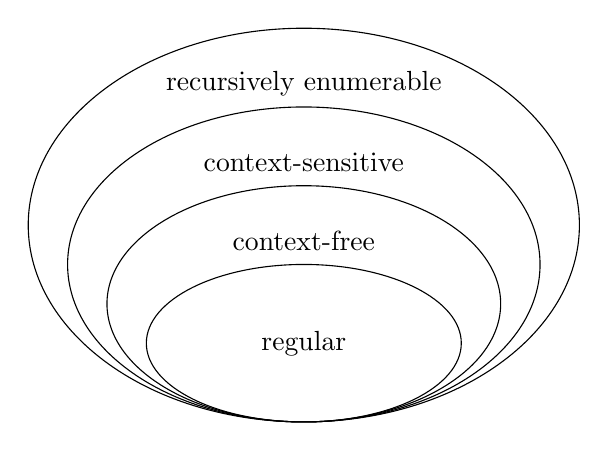
\begin{tikzpicture}
        %TODO: add colours to ellipses without overlapping
        \draw (0,0) ellipse (2 and 1);
        \draw (0,0.5) ellipse (2.5 and 1.5);
        \draw (0,1) ellipse (3 and 2);
        \draw (0,1.5) ellipse (3.5 and 2.5);
        \node at (0,0) {regular};
        \node at (0,1.3) {context-free};
        \node at (0,2.3) {context-sensitive};
        \node at (0,3.3) {recursively enumerable};
    \end{tikzpicture}
    \caption{Chomsky hierarchy of formal languages}
    \label{fig:chomsky-hierarchy}
\end{figure}


\subsubsection{Practical Implications}
The theoretical constructs discussed above are not only of academic interest but also have significant practical applications:
\begin{itemize}
    \item \textbf{Regular Expressions}: Extensively used in text processing (e.g., in tools such as \texttt{grep} and in lexical analysers) \cite{kernighan1984unix}.
    \item \textbf{Context-Free Grammars}: Form the basis for defining the syntax of programming languages such as Python and Java \cite{rozenberg1997handbook}.
    \item \textbf{Closure Properties}: Provide a framework for proving decidability results (e.g., the emptiness problem for \glspl{dfa}) \cite{sipser2013introduction}.
    \item \textbf{Probabilistic Models}: Applied in natural language processing and speech recognition for uncertainty modeling \cite{droste2009handbook}.
\end{itemize}
\subsection{\glsentrylongpl{cfa} Definition Fundamentals}
\label{subsec:automata-definition-fundamentals}

All automata share several core structural components that provide the basis for their computational behavior \cite{hopcroft2006introduction, sipser2013introduction}.

\begin{definition}[\glsentrylong{cfa}]
\label{def:finite-automaton}
A \textit{finite automaton} is a computational model that processes input symbols to recognise languages. Formally, a finite automaton $M$ is a quintuple $(Q, \Sigma, \delta, q_0, F)$, where:
\begin{itemize}
    \item \textbf{States ($Q$)}: A finite set of configurations representing the progress of computation \cite{sipser2013introduction}.
    \item \textbf{Input Alphabet ($\Sigma$)}: A finite set of symbols that the automaton processes \cite{hopcroft2006introduction, sudkamp2006languages}.
    \item \textbf{Transition Function ($\delta$)}: A function that governs state changes based on input. For deterministic models, $\delta: Q \times \Sigma \to Q$ is a total function (defined for all state-symbol pairs); for nondeterministic models, $\delta: Q \times \Sigma \to 2^Q$ \cite{sipser2013introduction}.
    \item \textbf{Initial State ($q_0 \in Q$)}: The starting configuration of the automaton \cite{hopcroft2006introduction}.
    \item \textbf{Accept States ($F \subseteq Q$)}: A subset of states indicating successful recognition of an input string \cite{sipser2013introduction}.
\end{itemize}
\end{definition}

\begin{remark}
The quintuple $(Q, \Sigma, \delta, q_0, F)$ provides a standardised representation for comparing automata models. The term "total function" in \glspl{dfa} means every state-symbol pair has exactly one transition \cite{sipser2013introduction}.
\end{remark}

\begin{example}
The \gls{dfa} in Figure~\ref{fig:cfa-example} is defined by:
\begin{itemize}
    \item $Q = \{q_0, q_1\}$,
    \item $\Sigma = \{0, 1\}$,
    \item Transitions: $\delta(q_0, 0) = q_0$, $\delta(q_0, 1) = q_1$, $\delta(q_1, 0) = q_1$, $\delta(q_1, 1) = q_0$,
    \item $F = \{q_0\}$, accepting strings with an even number of 1s.
\end{itemize}
\end{example}

\begin{figure}[htbp]
    \centering
    \begin{tikzpicture}[->,>=stealth,shorten >=1pt,auto,node distance=3cm,
                        semithick, every state/.style={minimum size=0.8cm}]
        % States
        \node[state, initial, accepting] (q0) {$q_0$};
        \node[state] (q1) [right=of q0] {$q_1$};
        
        % Transitions
        \path 
            (q0) edge [loop above] node {0} (q0)
                 edge [bend left=20] node {1} (q1)
            (q1) edge [loop above] node {0} (q1)
                 edge [bend left=20] node {1} (q0);
    \end{tikzpicture}
    \caption{\gls{dfa} recognizing strings with an even number of 1s. The double circle indicates the accept state $q_0$.}
    \label{fig:cfa-example}
\end{figure}

\begin{observation}
Graphical representations provide an intuitive understanding of automata behavior \cite{kozen1997automata, sudkamp2006languages}. 
Key conventions include:
\begin{itemize}
    \item \textbf{States}: Circles labeled with state names (e.g., $q_0$).
    \item \textbf{Initial State}: Marked by an unlabeled incoming arrow.
    \item \textbf{Accept States}: Double circles (e.g., $q_0$ in Figure~\ref{fig:cfa-example}).
    \item \textbf{Transitions}: Arrows labeled with input symbols.
\end{itemize}
\end{observation}

\begin{table}[htbp]
    \centering
    \begin{adjustbox}{max width=\textwidth}
      \begin{tabular}{@{}lllll@{}}
          \toprule
          \textbf{Automaton} & \textbf{Memory} & \textbf{Transitions} & \textbf{Acceptance Condition} & \textbf{Reference} \\ \midrule
          \gls{dfa} & None & Deterministic & Final state & \cite{sipser2013introduction} \\
          \gls{nfa} & None & Nondeterministic & Any accepting path & \cite{hopcroft2006introduction} \\
          \gls{pda} & Stack & Nondeterministic & Final state or empty stack & \cite{sipser2013introduction} \\
          \gls{tm} & Infinite tape & Deterministic & Halting in accept state & \cite{turing1936computable} \\
          \bottomrule
      \end{tabular}
    \end{adjustbox}
    \caption{Automata variations: structural and operational differences}
    \label{tab:automata-variations}
\end{table}

\subsection{Deterministic Finite Automata (DFA)}
\label{subsec:dfa} 

As a specialization of the general finite automaton framework~\ref{def:finite-automaton} established in Section~\ref{subsec:shared-foundations}, a Deterministic Finite Automaton (DFA)\cite{hopcroft2006introduction} is formally defined as a quintuple \( M = (Q, \Sigma, \delta, q_0, F) \) where:
\begin{itemize}
    \item \( Q \): Finite set of states
    \item \( \Sigma \): Finite input alphabet
    \item \( \delta: Q \times \Sigma \rightarrow Q \): Total transition function
    \item \( q_0 \in Q \): Unique initial state
    \item \( F \subseteq Q \): Set of accepting states
\end{itemize}

\subsubsection{Language Recognition and Expressive Power}
DFAs precisely characterize the class of regular languages (\(\mathsf{REG}\)) within the Chomsky hierarchy \cite{hopcroft2006introduction}. Key properties include:

\begin{enumerate}
    \item \textbf{Closure Properties}: Closed under union, intersection, complement, concatenation, and Kleene star \cite{myhill1957finite}.
    \item \textbf{Limitations}: Cannot recognize non-regular languages like \( \{a^nb^n | n \geq 0\} \) (pumping lemma consequence) \cite{sipser2012introduction}.
    \item \textbf{Equivalence}: All regular expressions have corresponding DFAs and vice versa (Kleene's theorem) \cite{kleene1956representation}.
\end{enumerate}

The Myhill-Nerode theorem provides a canonical minimal DFA for any regular language, establishing state minimality criteria \cite{nerode1958linear}.

\subsubsection{Graphical Representation}
Consider the DFA in Figure~\ref{fig:dfa-example} recognizing strings with an even number of \texttt{0}s and \texttt{1}s. The automaton transitions between states based on input symbols, accepting strings that satisfy the parity constraints.

\begin{figure}[h]
    \centering  
    \begin{tikzpicture}[shorten >=1pt, node distance=3cm, on grid, auto]
        \node[state, initial, accepting, initial text={}] (q0) {$q_0$};
        \node[state] (q1) [right=of q0] {$q_1$};
        \node[state] (q2) [below=of q1] {$q_2$};
        \node[state] (q3) [left=of q2] {$q_3$};

        \path[->]
        (q0) edge [bend left] node {1} (q1)
        (q0) edge [bend right] node[swap] {0} (q3)
        (q1) edge [bend right] node[swap] {0} (q2)
        (q1) edge [bend left] node {1} (q0)
        (q2) edge [bend left] node {1} (q3)
        (q2) edge [bend right] node[swap] {0} (q1)
        (q3) edge [bend right] node[swap] {0} (q0)
        (q3) edge [bend left] node {1} (q2);
    \end{tikzpicture}
    \caption{DFA recognizing even numbers of \texttt{0}s and \texttt{1}s.}
    \label{fig:dfa-example}
\end{figure}

\(
L = \{ w \in \{0, 1\}^* \mid \text{the number of } 0\text{'s in } w \text{ is even and the number of } 1\text{'s in } w \text{ is even} \}
\) is the language recognized by this DFA.

The DFA is deterministic because for each state and input symbol (either \texttt{0} or \texttt{1}), there is exactly one transition defined. This ensures that from any given state, the next state is uniquely determined by the current input symbol, leaving no ambiguity in the automaton's behavior.

The structure of the DFA ensures that it keeps track of the parity (even or odd) of the counts of \texttt{0}s and \texttt{1}s as it processes each input symbol, transitioning between states accordingly to accept only those strings that meet the specified criteria.


\subsection{\acrfull{nfa}}
\label{subsec:nfa}

\begin{definition}[\gls{nfa}]
A \gls{nfa} is a quintuple 
\[
M = (Q, \Sigma, \delta, q_0, F)
\]
where:
\begin{itemize}
    \item \( Q \) is a finite set of states,
    \item \( \Sigma \) is an input alphabet,
    \item \( \delta: Q \times (\Sigma \cup \{\epsilon\}) \rightarrow 2^Q \) is a nondeterministic transition function,
    \item \( q_0 \in Q \) is the initial state, and
    \item \( F \subseteq Q \) is the set of accepting states.
\end{itemize}
\end{definition}

\begin{remark}
Unlike \glspl{dfa}, a \gls{nfa} may have multiple transitions for a given state and input symbol, including transitions on the empty string \(\epsilon\). This nondeterminism allows for multiple computational paths.
\end{remark}

\begin{example}
Figure~\ref{fig:nfa-example} depicts a \gls{nfa} that recognises the language 
\[
L = \{ w \in \{a,b\}^* \mid w \text{ contains the substring } ab \}.
\]
\end{example}

\begin{algorithm}[Subset Construction for \glspl{nfa}]
\label{alg:subset}
To convert an \gls{nfa} \( N = (Q, \Sigma, \delta, q_0, F) \) into an equivalent \gls{dfa}:
\begin{enumerate}
    \item Compute the \(\epsilon\)-closure of the initial state: \( S_0 = \epsilon\text{-closure}(\{q_0\}) \).
    \item For each \gls{dfa} state \( S \subseteq Q \) and each input symbol \(\sigma \in \Sigma\), define 
    \[
    \delta_{\text{\gls{dfa}}}(S, \sigma) = \epsilon\text{-closure}\Big(\bigcup_{q \in S} \delta(q, \sigma)\Big).
    \]
    \item Mark \( S \) as accepting if \( S \cap F \neq \emptyset \).
    \item Repeat until no new states are produced.
\end{enumerate}
\end{algorithm}

\begin{observation}
The subset construction algorithm may produce up to \(2^{|Q|}\) states in the worst case, illustrating a potential state explosion when converting an \gls{nfa} to a \gls{dfa}.
\end{observation}

\begin{figure}[h]
    \centering  
    \begin{tikzpicture}[shorten >=1pt, node distance=2.5cm, on grid, auto]
        \node[state, initial, initial text={}] (q0) {$q_0$};
        \node[state] (q1) [right=of q0] {$q_1$};
        \node[state, accepting] (q2) [right=of q1] {$q_2$};

        \path[->]
        (q0) edge [loop above] node {$a,b$} (q0)
        (q0) edge node {$a$} (q1)
        (q1) edge node {$b$} (q2);
    \end{tikzpicture}
    \caption{NFA recognizing \( L = \Sigma^*ab \)}
    \label{fig:nfa-example}
\end{figure}

\begin{figure}[h]
    \centering  
    \begin{tikzpicture}[shorten >=1pt, node distance=3cm, on grid, auto]
        \node[state, initial, initial text={}] (A) {$\{q_0\}$};
        \node[state] (B) [right=of A] {$\{q_0, q_1\}$};
        \node[state, accepting] (C) [right=of B] {$\{q_0, q_2\}$};

        \path[->]
        (A) edge [loop below] node {$b$} (A)
        (A) edge node {$a$} (B)
        (B) edge [loop below] node {$a$} (B)
        (B) edge node {$b$} (C)
        (C) edge [bend left] node {$a$} (B)
        (C) edge [bend right] node[swap] {$b$} (A);
    \end{tikzpicture}
    \caption{Equivalent DFA for NFA in Figure~\ref{fig:nfa-example} \cite{hopcroft2006introduction}}
    \label{fig:dfa-conversion}
\end{figure}
\subsection{Probabilistic Finite Automata (PFA)}
\label{subsec:pfa}

As a generalization of the classical finite automaton framework~\ref{def:finite-automaton} established in Section~\ref{subsec:shared-foundations}, a Probabilistic Finite Automaton (PFA)\cite{rabin1963probabilistic} is formally defined as a quintuple \( M = (Q, \Sigma, \delta, \pi, F) \) where:
\begin{itemize}
    \item \( Q \): Finite set of states
    \item \( \Sigma \): Finite input alphabet
    \item \( \delta: Q \times \Sigma \times Q \rightarrow [0,1] \): Probabilistic transition function satisfying \( \sum_{q' \in Q} \delta(q, \sigma, q') = 1 \) for all \( q \in Q \), \( \sigma \in \Sigma \)
    \item \( \pi \in \mathbb{R}^{|Q|} \): Initial state distribution vector with \( \sum_{q \in Q} \pi_q = 1 \)
    \item \( F \subseteq Q \): Set of accepting states
\end{itemize}

\subsubsection{Language Recognition and Expressive Power}
PFAs recognize stochastic languages through probabilistic acceptance criteria. The language recognized by a PFA \( M \) with cut-point \( \lambda \in [0,1) \) is:
\[ L(M, \lambda) = \{ w \in \Sigma^* \mid \Pr[M \text{ accepts } w] > \lambda \} \]

Key variants and their properties include:

\begin{enumerate}
    \item \textbf{Isolated Cut-Point (\( \lambda \) with margin \( \epsilon > 0 \))}:
    \[ \Pr[M \text{ accepts } w] \begin{cases} 
    \geq \lambda + \epsilon & \text{if } w \in L \\
    \leq \lambda - \epsilon & \text{if } w \notin L 
    \end{cases} \]
    Recognizes exactly the regular languages \cite{rabin1963probabilistic}
    
    \item \textbf{Non-Isolated Cut-Point (\( \lambda = 0 \))}:
    \[ L(M, 0) = \{ w \mid \Pr[M \text{ accepts } w] > 0 \} \]
    Recognizes languages beyond regular, including context-sensitive \cite{paz1971introduction}
    
    \item \textbf{Strict Cut-Point (\( \lambda = 1 \))}:
    \[ L(M, 1) = \{ w \mid \Pr[M \text{ accepts } w] = 1 \} \]
    Equivalent to deterministic finite automata \cite{salomaa1969probabilistic}
\end{enumerate}

\subsubsection{Closure Properties}
PFAs exhibit nuanced closure characteristics compared to classical models:
\begin{itemize}
    \item Closed under union, intersection, and reversal \cite{paz1971introduction}
    \item \textbf{Not closed} under complementation unless using isolated cut-points \cite{bertoni1994closure}
    \item Kleene star closure requires additional constraints on transition probabilities \cite{hromkovic2000probabilistic}
\end{itemize}

\subsubsection{Graphical Representation}
Consider a PFA recognizing \( L_{\text{maj}} = \{ w \in \{a,b\}^* \mid |w|_a > |w|_b \} \) with probability \( \geq 2/3 \):

\begin{figure}[h]
    \centering  
    \begin{tikzpicture}[shorten >=1pt, node distance=3cm, on grid, auto]
        \node[state, initial, initial text={$\pi=1$}] (q0) {$q_0$};
        \node[state, accepting] (q1) [right=of q0] {$q_1$};
        
        \path[->]
        (q0) edge [loop above] node {a(0.6), b(0.4)} (q0)
        (q0) edge [bend left] node {a(0.4), b(0.6)} (q1)
        (q1) edge [loop above] node {a(0.3), b(0.7)} (q1)
        (q1) edge [bend left] node {a(0.7), b(0.3)} (q0);
    \end{tikzpicture}
    \caption{PFA for majority language with probabilistic transitions}
    \label{fig:pfa-example}
\end{figure}

This PFA maintains a probability distribution across states, with transitions weighted by input symbol probabilities. Acceptance occurs when the cumulative probability in \( F \) exceeds the cut-point after processing the entire input.

\subsubsection{Key Theoretical Results}
\begin{enumerate}
    \item \textbf{Rabin's Theorem}: PFAs with isolated cut-points recognize exactly \(\mathsf{REG}\) \cite{rabin1963probabilistic}
    \item \textbf{Pumping Lemma}: Probabilistic version requires probability bounds on loop iterations \cite{paz1971introduction}
    \item \textbf{Equivalence Problem}: Undecidable for PFAs with non-isolated cut-points \cite{tzelepis2021undecidable}
\end{enumerate}
%%%%%%%%%%%%%%%%%%%%%%%%%%%%%%%%%%%%%%%%%%%%%%%%%%%%%%%%%%%%%%%
% Two-Way Finite Automata Variants
%%%%%%%%%%%%%%%%%%%%%%%%%%%%%%%%%%%%%%%%%%%%%%%%%%%%%%%%%%%%%%%

\subsection{Two-Way Finite Automata Variants}
\label{subsec:two-way-variants}

Two-way finite automata extend the classical one‐way model by allowing the read head to move in both directions over the input. Although this extra power does not increase the class of recognizable languages (both one‐way and two‐way automata recognize exactly the regular languages), two‐way models can be exponentially more succinct than one‐way models and naturally lend themselves to algorithms in several contexts (e.g., in complexity analysis and even quantum models).

%%%%%%%%%%%%%%%%%%%%%%%%%%%%%%%%%%%%%%%%%%%%%%%%%%%%%%%%%%%%%%%
% Two-Way Deterministic Finite Automata (2DFA)
%%%%%%%%%%%%%%%%%%%%%%%%%%%%%%%%%%%%%%%%%%%%%%%%%%%%%%%%%%%%%%%

\subsubsection{\acrfull{2dfa}}
\label{subsubsec:2dfa}

\begin{definition}[Two-Way Deterministic Finite Automaton]
A \gls{2dfa} is formally defined as an 8-tuple 
\[
M = (Q, \Sigma, L, R, \delta, s, t, r),
\]
where:
\begin{itemize}
  \item \(Q\) is a finite set of states,
  \item \(\Sigma\) is a finite input alphabet,
  \item \(L\) and \(R\) are special symbols called the left and right endmarkers, respectively (with \(L,R \notin \Sigma\)),
  \item \(\delta: Q \times (\Sigma \cup \{L, R\}) \to Q \times \{L, R\}\) is the transition function,
  \item \(s\in Q\) is the start state,
  \item \(t\in Q\) is the (unique) accept state, and
  \item \(r\in Q\) (with \(r\neq t\)) is the (unique) reject state.
\end{itemize}
In addition, the transition function is assumed to satisfy:
\begin{itemize}
  \item For every state \(q\in Q\), when reading the left endmarker \(L\), the head always moves to the right; that is, \(\delta(q,L) = (q', R)\) for some \(q'\in Q\).
  \item Similarly, when reading the right endmarker \(R\), the head always moves to the left: \(\delta(q,R) = (q', L)\).
  \item Once the machine reaches the accept state \(t\) (or the reject state \(r\)), it remains there (the transition always maps back to itself) while moving in a fixed direction.
\end{itemize}
\end{definition}

\begin{remark}
The two-way motion allows the automaton to perform multiple passes over the input, which can result in an exponential reduction in the number of states compared to one-way automata, though at the expense of increased operational complexity.
\end{remark}

\begin{example}[First and Last Symbol Equality]
Consider the language 
\[
L = \{ w\in \{0,1\}^* \mid \text{the first symbol of } w \text{ equals the last symbol} \}.
\]
A \gls{2dfa} for \(L\) operates as follows:
\begin{enumerate}
  \item Start at the left endmarker \(L\) and immediately move right to read the first symbol; store it in the control.
  \item Continue scanning right until the right endmarker \(R\) is reached.
  \item Upon reading \(R\), reverse direction (move left) and, in the process, skip any blank moves until the last symbol is reached.
  \item Compare the stored first symbol with the last symbol. If they are equal, move to the accept state \(t\); otherwise, move to the reject state \(r\).
\end{enumerate}
A simplified state diagram illustrating this process is provided in Figure~\ref{fig:2dfa-example}.
\end{example}

\begin{observation}
Although every \gls{2dfa} can be simulated by a one-way \gls{dfa}, such a simulation may require an exponential increase in the number of states.
\end{observation}

\paragraph{Operational Mechanics}
The two-way motion enables the automaton to make multiple passes over the input, which is particularly useful for verifying properties that depend on both the prefix and the suffix of the input string.

\paragraph{State Complexity and Conversion Algorithms}
For some families of regular languages, \glspl{2dfa} can be exponentially more succinct than their one-way counterparts. Conversion algorithms—such as those proposed by Shepherdson and Kozen—use crossing sequences to simulate two-way behavior in a one-way \gls{dfa}, typically at the cost of exponential state blow-up.

%%%%%%%%%%%%%%%%%%%%%%%%%%%%%%%%%%%%%%%%%%%%%%%%%%%%%%%%%%%%%%%
% Two-Way Nondeterministic Finite Automata (2NFA)
%%%%%%%%%%%%%%%%%%%%%%%%%%%%%%%%%%%%%%%%%%%%%%%%%%%%%%%%%%%%%%%

\subsubsection{\acrfull{2nfa}}
\label{subsubsec:2nfa}

\begin{definition}[Two-Way Nondeterministic Finite Automaton]
A \gls{2nfa} is defined similarly to a \gls{2dfa} but with a nondeterministic transition function. Formally, a \gls{2nfa} is an 8-tuple
\[
M = (Q, \Sigma, L, R, \delta, s, t, r),
\]
where:
\begin{itemize}
    \item \(Q\) is a finite set of states,
    \item \(\Sigma\) is a finite input alphabet,
    \item \(L\) and \(R\) are the left and right endmarkers (with \(L,R\notin\Sigma\)),
    \item \(\delta: Q \times (\Sigma \cup \{L,R\}) \to 2^{\,Q \times \{L,R\}}\) is the nondeterministic transition function,
    \item \(s\in Q\) is the start state,
    \item \(t\in Q\) is the unique accept state, and
    \item \(r\in Q\) (with \(r\neq t\)) is the unique reject state.
\end{itemize}
The transition function obeys similar boundary conditions as in the \gls{2dfa} case.
\end{definition}

\begin{remark}
The nondeterminism in a \gls{2nfa} allows it to "guess" important positions within the input and verify them via bidirectional traversal, which can lead to significant state savings compared to deterministic models.
\end{remark}

\begin{example}[Symmetry Check (Toy Version)]
Consider the language 
\[
L_{sym} = \{ w \in \{0,1\}^* \mid \text{the first two symbols equal the last two symbols} \}.
\]
A high-level description of a \gls{2nfa} for \(L_{sym}\) is:
\begin{enumerate}
    \item Scan right from the left endmarker \(L\) while nondeterministically guessing the point where comparison will occur.
    \item Upon reaching the right endmarker \(R\), reverse direction.
    \item While moving left, nondeterministically check that the stored first two symbols match the corresponding symbols at the end.
    \item If both comparisons succeed, transition to the accept state \(t\); otherwise, transition to the reject state \(r\).
\end{enumerate}
Figure~\ref{fig:2nfa-example} schematically illustrates this guess-and-check mechanism.
\end{example}

\begin{observation}
\glspl{2nfa} can be exponentially more succinct than one-way \glspl{dfa}, even though the class of languages they recognize remains the same (i.e., the regular languages).
\end{observation}

%%%%%%%%%%%%%%%%%%%%%%%%%%%%%%%%%%%%%%%%%%%%%%%%%%%%%%%%%%%%%%%
% Two-Way Probabilistic Finite Automata (2PFA)
%%%%%%%%%%%%%%%%%%%%%%%%%%%%%%%%%%%%%%%%%%%%%%%%%%%%%%%%%%%%%%%

\subsubsection{\acrfull{2pfa}}
\label{subsubsec:2pfa}

\begin{definition}[Two-Way Probabilistic Finite Automaton]
A \gls{2pfa} is an 8-tuple
\[
M = (Q, \Sigma, L, R, \delta, s, t, r),
\]
where:
\begin{itemize}
    \item \(Q\) is a finite set of states,
    \item \(\Sigma\) is a finite input alphabet,
    \item \(L\) and \(R\) are the left and right endmarkers (with \(L,R \notin \Sigma\)),
    \item \(\delta: Q \times (\Sigma \cup \{L,R\}) \to \mathbb{R}_{\ge 0}^{\,Q \times \{L,R\}}\) is a probabilistic transition function such that
    \[
    \sum_{(q',d)\in Q\times\{L,R\}} \delta(q,a,q',d) = 1 \quad \text{for all } q \in Q \text{ and } a \in \Sigma \cup \{L,R\},
    \]
    \item \(s\in Q\) is the start state,
    \item \(t\in Q\) is the unique accept state, and
    \item \(r\in Q\) (with \(r\neq t\)) is the unique reject state.
\end{itemize}
\end{definition}

\begin{remark}
A \gls{2pfa} extends the probabilistic finite automaton by allowing bidirectional head movement. Its transitions are governed by probability distributions, and acceptance is determined by whether the cumulative probability of reaching the accept state exceeds a predetermined cut-point.
\end{remark}

\begin{example}[Majority Language]
Consider the language 
\[
L_{maj} = \{ w \in \{a,b\}^* \mid \#a(w) > \#b(w) \}.
\]
A \gls{2pfa} for \(L_{maj}\) operates by making probabilistic passes over the input, updating state probabilities, and eventually halting in the accept state \(t\) if the acceptance probability is high enough. Figure~\ref{fig:2pfa-example} provides a schematic illustration of such a machine.
\end{example}

\begin{theorem}[Rabin's Theorem for \glspl{pfa}]
\label{thm:2pfa-rabin}
A \gls{pfa} with an isolated cut-point recognizes exactly the class of regular languages. This result extends to \glspl{2pfa} under analogous conditions.
\end{theorem}

\begin{proposition}
If a \gls{2pfa} employs a non-isolated cut-point (e.g., \(\lambda = 0\)), it may recognize languages beyond the regular class.
\end{proposition}

\begin{corollary}
For a \gls{2pfa} with a strict cut-point (\(\lambda = 1\)), the recognized language is equivalent to that of a \gls{dfa}.
\end{corollary}

%%%%%%%%%%%%%%%%%%%%%%%%%%%%%%%%%%%%%%%%%%%%%%%%%%%%%%%%%%%%%%%
% Comparative Analysis of Two-Way Models
%%%%%%%%%%%%%%%%%%%%%%%%%%%%%%%%%%%%%%%%%%%%%%%%%%%%%%%%%%%%%%%

\subsubsection{Comparative Analysis of Two-Way Models}
\label{subsubsec:two-way-comparison}

\begin{table}[h]
    \centering
    \begin{adjustbox}{max width=\textwidth}
    \begin{tabular}{|l|c|c|c|c|l|}
        \hline
        \textbf{Model} & \textbf{Language Class} & \textbf{Time Complexity} & \textbf{Space Complexity} & \textbf{State Complexity} & \textbf{Key Reference} \\
        \hline
        \gls{2dfa}  & REG & \(O(n^2)\) & \(O(1)\) & May be exponentially smaller than 1DFA & \cite{hopcroft2006introduction} \\
        \gls{2nfa}  & REG & \(O(n)\) & \(O(1)\) & Can be exponentially more succinct than 1DFA & \cite{yakaryilmaz2010succinctness} \\
        \gls{2pfa}  & \( \mbox{REG} \subset L \subseteq \mbox{P} \) & \(O(n^3)\) & \(O(\log n)\) & Varies with error bounds & \cite{freivalds1981probabilistic} \\
        \hline
    \end{tabular}
    \end{adjustbox}
    \caption{Comparison of classical two-way automata models (using explicit endmarkers).}
    \label{tab:two-way-comparison}
\end{table}

\begin{remark}
The comparative analysis illustrates that while all two-way automata recognize only regular languages, the two-way models often achieve significant advantages in state complexity and, in some cases, time complexity, compared to their one-way counterparts.
\end{remark}

\begin{center}
\begin{tikzpicture}[shorten >=1pt,node distance=2.5cm,on grid,auto]
  \node[state,initial,accepting] (q0) {\(q_0\)};
  \node[state] (q1) [right=of q0] {\(q_1\)};
  \node[state] (q2) [below=of q1] {\(q_2\)};
  \node[state,accepting] (t) [left=of q2] {\(t\)};
  \node[state,rejecting] (r) [below=of q0] {\(r\)};

  \path[->]
    (q0) edge node {read first symbol, store \(a\)} (q1)
    (q1) edge [bend left] node {scan right until \(R\)} (q2)
    (q2) edge [bend left] node {reverse; on \(R\) switch to leftward} (q1)
    (q2) edge node {at last symbol, compare with \(a\)} (t)
    (q2) edge [bend right] node [swap] {if mismatch} (r);
\end{tikzpicture}
\end{center}

\begin{figure}[h]
    \centering  
    \begin{tikzpicture}[shorten >=1pt, node distance=2cm, on grid, auto]
        \node[state, initial] (q0) {\(q_0\)};
        \node[state] (q1) [right=of q0] {\(q_1\)};
        \node[state, accepting] (q2) [right=of q1] {\(q_2\)};
        \node[state, rejecting] (qr) [below=of q1] {\(r\)};
        \path[->]
            (q0) edge [loop above] node {\(0,1,R\)} (q0)
            (q0) edge node {\(\triangleright\)} (q1)
            (q1) edge [loop above] node {\(0,1,L\)} (q1)
            (q1) edge [bend left] node {\(0/1\)} (q2)
            (q1) edge [bend right] node[swap] {\(0/1\)} (qr);
    \end{tikzpicture}
    \caption{Schematic 2NFA illustrating a guess-and-check mechanism (for a toy symmetry language).}
    \label{fig:2nfa-example}
\end{figure}

\begin{figure}[h]
    \centering  
    \begin{tikzpicture}[shorten >=1pt, node distance=2.5cm, on grid, auto]
        \node[state, initial] (q0) {\(q_0\)};
        \node[state] (q1) [right=of q0] {\(q_1\)};
        \node[state, accepting] (q2) [right=of q1] {\(q_2\)};
        \path[->]
            (q0) edge [loop above] node[align=center] {\(a:0.6R\)\\\(b:0.4R\)} (q0)
            (q0) edge node {\(\triangleright:0.5\)} (q1)
            (q1) edge [loop above] node[align=center] {\(a:0.3L\)\\\(b:0.7L\)} (q1)
            (q1) edge node {\(\triangleleft:0.7\)} (q2);
    \end{tikzpicture}
    \caption{Schematic 2PFA for a majority language (with sample probabilistic transitions).}
    \label{fig:2pfa-example}
\end{figure}
